
\chapter{Data Lineage Analysis for Frameworks \label{chapter:implementation}}

In Chapter \ref{chapter:frameworks} we described Java frameworks
that are often used in applications to manipulate with data.

In Section \ref{frameworks:requirements} we described the key requirements
on the library to analyse data lineage of such applications.
The analysis library should:
\begin{itemize}
  \item Identify the data sources and sinks.
  \item Create correct and accurate data lineage in reasonable time.
  \item Work with the concrete values for Java primitives and \Code{String}s.
  \item Work with external files.
  \item Support for the callback objects.
  \item Be easily extendible to support new frameworks.
\end{itemize}

In Section \ref{chapter:analysis:symbolicAnalysisLibrary} we described the
static program analysis approach used by the existing library
for creating data lineage of plain Java programs.
Using that library, data lineage can be created for Java I/O and JDBC API.

In this chapter, we will present our solution of data lineage analysis
for database frameworks - the \ToolName tool.
The \ToolName tool uses the Symbolic analysis library, which takes
care of the data flow propagation between sources and sinks.
The \ToolName tool implements features for identifying the sources
and sinks of data inside frameworks as plugins to the Symbolic analysis library.

We will discuss the design of the \ToolName tool and some technical details
of implemented Symbolic analysis library plugins.




\section{Symbolic Analysis Library Plugins}

In this section we describe the main ideas about plugin approach of our \ToolName tool.

When the Symbolic analysis library performs the program analysis,
the plugin handles the selected method calls on frameworks and provides
information about the data sources and data sinks to the library.

An input of a plugin is computed data flow information
about the receiver (\Code{this} object) and the method call arguments.
The Section \ref{chapter:analysis:algorithm} describes the Symbolic analysis algorithm
as iterative updating of method summaries until a fixpoint is reached.

The same approach applies for the plugins. At each iteration, the flow information
about the plugin inputs are computed by the library and based on their values,
plugin provides information about the data sources and sinks of a framework method call.




\section{Interface to Symbolic Analysis \label{chapter:implementation:interface}}

We proposed the general interface between Symbolic analysis library and its plugins.
Communication between the library and plugins is described in
Figure \ref{implementation:analysis-plugins-communication}.

\begin{figure}[p]
  \centering
  % trim - left lower right upper
  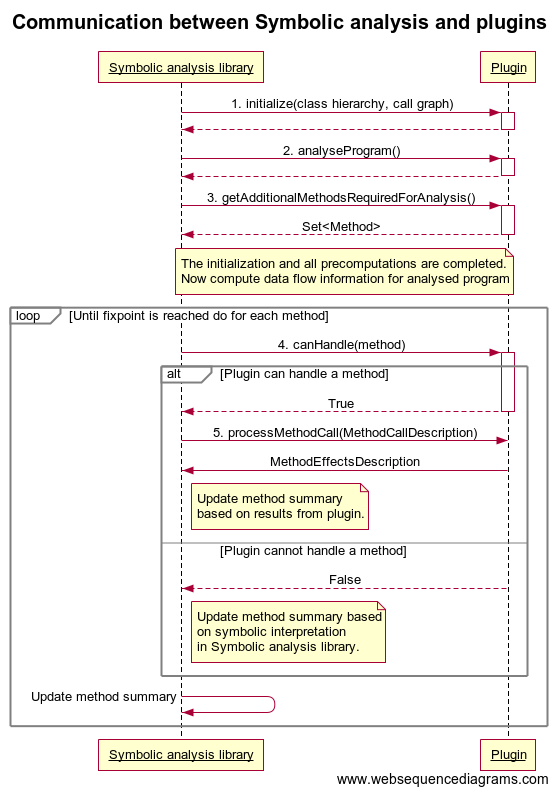
\includegraphics[trim={0cm 0.75cm 0cm 1.4cm},clip,width=\textwidth]{img/analysis-plugins-communication.png}
  \caption{Communication between Symbolic analysis and the plugins}
  \label{implementation:analysis-plugins-communication}
\end{figure}

In next sections we will describe all the interfaces used between the library and the plugins.



\subsection{FrameworkAnalysisPlugin}

The key interface for plugin to Symbolic analysis library is the \Code{Framework\-AnalysisPlugin}.
The interface defines few methods that are used for communication between the library and plugins.
Here we describe their usage:
\begin{itemize}
  \item \Code{initialize} and \Code{analyzeProgram} initialize plugins
    and precompute some information from the provided call graph and class hierarchy
    of an analysed program.
  \item \Code{getAdditionalMethodsRequiredForAnalysis} specify framework methods that should
    be also analysed by the Symbolic analysis library, as the library does not
    analyse methods out of defined application package because of optimizations.
    Sometime it is useful to analyse other framework methods
    (e.g. when there are many overloading methods that forward their calls to one method
    that can be handled by a plugin).
  \item \Code{canHandleMethod} and \Code{processMethodCall} query plugin whether method can be
    handled by the plugin and to compute flow information for such method.
  \item \Code{canProvideArgument} and \Code{getArgumentFlowInformation} provide flow information for
    an argument of a callback method.
  \item \Code{destroy} closes all plugin resources. The method is used at the end of analysis,
    when the fixpoint is reached.
\end{itemize}




\subsection{MethodCallDescription}

The class \Code{MethodCallDescription} serves as data flow information input for a plugin query
(the \Code{processMethodCall} method).
It holds the attributes for all method inputs
(for receiver (\Code{this} object) and all the method arguments)
and also flow information about the previously analysed callbacks.




\subsection{MethodEffectsDescription}

The class \Code{MethodEffectsDescription} serves as output of the
\Code{processMethodCall} method. It holds the output data flow information
and also identifies callbacks to be computed by the Symbolic analysis library.

Flow information are stored in the \Code{DataEndpointFlowInfo} object that
is described in the next section.



\subsection{DataEndpointFlowInfo}

The class \Code{DataEndpointFlowInfo} holds data flow information results
for an analysed method, such as:
\begin{itemize}
  \item Identification of the data source or sink.
  \item Mapping of fields in the resulting objects to data source or sink information (e.g. database column name)
    The results can be returned by a method and also stored into a method attribute.
  \item Attributes for:
    \begin{itemize}
      \item Data source or sink
      \item Returned object
      \item Receiver (\Code{this})
      \item Method call arguments
    \end{itemize}
\end{itemize}

The data source and sink identification can be the SQL statement in case of database frameworks,
or the server identification or other information.

Plugin can define its own attributes that can be used to identify any valuable information.
All of the attributes are then propagated using the Symbolic analysis library.




\section{JDBC API \label{implementation:jdbc}}

Implementation of Data Lineage for standard JDBC API in \Code{java.sql} package
is done using the Symbolic analysis library, as we show in the Section \ref{chapter:analysis:symbolicAnalysisLibrary}.

In this section we will describe our solution for \Code{DataSource} interfaces in \Code{javax.sql} package.
It is nowadays the preferred way of creating connections to database and the Symbolic Analysis
library do not handle such information.



\subsection{DataSource \label{implementation:dataSource}}

Database vendors usually provide \Code{DataSource} implementation, which still
needs some configuration about database - connection url, credentials and probably much more.

To identify target database, we need information about connection url and credentials. These properties
are usually set to \Code{DataSource} objects and from these calls, we can get
their values.

The plugins identify the methods where such information is set and return
the concrete values of used \Code{String}s for propagation by Symbolic analysis library.



\section{Spring JDBC Framework}

Spring JDBC Framework comes with approach of callbacks. It handles
all boilerplate code and calls user defined callback objects to do their job
and after finishing it, framework handles closing all resources that are not needed anymore.

When we looked to implementation of \Code{JdbcTemplate} class, we found out
that database calls are actually made only by 4 out of about 50 of its methods.
All the other methods only use them when executing queries.



\subsection{Callbacks}

As we said, callbacks are used just to wrap application logic and
separate it from the code for opening/closing connections, etc,
as was shown by previous example \ref{code:jdbcTemplate}.

When handling a particular method of the framework (e.g. the \Code{update}
method of \Code{JdbcTemplate} class in Listing \Code{code:jdbcTemplate}),
we needed to find a way how to say to the Symbolic analysis library that a plugin wants to
analyse that callback method. For that purpose, we use
field \Code{callbackMethodsToAnalyze} from interface.
All callbacks have the method that is called in execution
and we just leave analysis library to analyse it and return
its data flow. After that, we append the resulting flow of the callback
to flow of our handled method.

We will demonstrate it on simple example of the \Code{insert} method from Listing \ref{code:jdbcTemplate}.
In the method, there is the call of the \Code{jdbcTemplate.update()} method
with two arguments - the SQL statement and the instance of \Code{PreparedStatementSetter}.

After data lineage analysis of the \Code{insert} method is done, we would like to know
that the \Code{id} and \Code{value} attributes of the \Code{DatabaseValue} instance
were arguments of the executed SQL statement.
However, Symbolic analysis library does not know that, inside of \Code{jdbcTemplate.update()},
the \Code{setValues} method of the \Code{PreparedStatementSetter} is called.

Our solution is that when the plugin is handling
\Code{jdbcTemplate.execute()} for the first time, it tells library
that it wants to analyse that \Code{setValues} call.
The next time the plugin already has all the information
about data lineage in the \Code{setValues}
and therefore it can propagate it to the result of the \Code{jdbcTemplate.update()} call.




\section{MyBatis}

In chapter \ref{frameworks:myBatis} we showed classic use case of loading data from database
using the MyBatis framework. Now, we present solution of computing data lineage for this framework.



\subsection{Mapper interfaces}

First, it is necessary to find all the mapper interfaces.
To do this, we iterate all classes in class hierarchy and search 
for interfaces with methods annotated with MyBatis annotations,
or interfaces for which XML mapper definition exists.



\subsubsection{XML mapper files}

XML mapper file definition has same name as the corresponding interface
(but .xml extension is used instead of .java), and lays in same directory.

We made a parser of such XML files that can get information about SQL statements
and mapping of columns to object fields.

Parser supports reusable SQL fragments. Each fragment has its own ID,
so it is easy to find correct one and include it into query.

Parser also supports dynamic SQLs. As we do not know which conditions are valid
at runtime, we made a simplification that we always use just first branch that
was seen in code.
We also cannot determine the size of an input collection, so the parser provides no expansion.



\subsubsection{Annotated mapper classes}

When mappers use annotations, it is quite simple to get all data needed
from WALA. We know that an SQL statement is always stored in annotations
\Code{@Select}, \Code{@Insert}, \Code{@Delete} or \Code{@Update}
and queries are stored in plain \Code{String} array.
Queries can also contain dynamic SQL as in XML definitions.

For mapping result object the \Code{@Results} annotation is used with \Code{@Result}
for every column to object property mapping definition.
Mapping can be done using \Code{@ConstructorArgs}, when columns are mapped
to arguments of a constructor. In that case, the plugin unfortunately does not know
the name of target property, as arbitrary code can be executed in constructor\footnote{
  Arbitrary code can be executed also in setters, but it is usually used
  just as setting new reference of a property.
}.

Framework can provide result of an SQL query in two ways:
\begin{enumerate}
  \item As a return statement of a mapper method.
  \item As a method argument property.
\end{enumerate}

In all previous mapper examples, we use the first approach, where result
is returned from method in return statement.

However, when calling database procedure, we can define its output arguments
and framework fill result values into that method argument.
It can be \Code{Map<String, Object>} object (where mapper references to key in that map),
or any arbitrary object (where mapper references field, in which result will be stored).

Listing \ref{code:mybatis:advanced:map} illustrates the use of such \Code{Map} as
input and also output method argument.
The database call of \Code{DB\_PROCEDURE} has two arguments.

First, the input integer argument, takes value of the \Code{id} key from the map.
Second, the output cursor argument, is created by MyBatis and perform database procedure call.
The cursor is then transformed to list of target object
with result map \Code{resultMap} and stored to the same map under the key \Code{result}.

\InsertCode{h}{code/mybatis-output-arguments.tex}

There also exist more advanced features of MyBatis when using annotations\footnote{
  Such as using provider classes to create SQL queries (\Code{@SelectProvider}, $\ldots$),
  generating IDs from sequence (\Code{@SelectKey}) and using them in queries,
  generating maps from objects (\Code{@MapKey}),
  associations for attribute classes (\Code{@One} or \Code{@Many}),
  mixing XML and annotation mappers (e.g. define \Code{<resultMap>} in XML and reference it
  using \Code{@ResultMap} annotation)}
but we do not handle them. All of them can be added as new functionality in future development,
if needed.




\subsection{Database connection configuration}

Configuration of MyBatis can be done in two ways, using XML configuration file
or in Java using \Code{Configuration} class. Second way needs no more attention,
as we use \Code{DataSource} classes that are already handled in section \ref{implementation:dataSource}.

To handle XML configuration, our plugin needs to parse configuration file and find \Code{<dataSource>}
section and its \Code{driver}, \Code{url} and \Code{username} properties. All this
information we need for identifying target database.




\section{Kafka}

In section \ref{frameworks:kafka} we demonstrated the main use cases
for data manipulation (producing or consuming) using Kafka framework.
In this section, we show how data lineage for these examples can be computed
using our plugin. In our work, we focused only on Consumer and Producer APIs,
as the other two (Stream and Connector APIs) are much more advanced to use.

The plugin identifies the used Kafka server which is used in application to communicate with.
It also identifies the methods that are used to set Kafka topics
and the methods that are used to send and receive a data.

Together, the used server, topic and the place where data are produced and consumed,
are the main data lineage information about the sources and sinks of a data.




\subsection{Callbacks}

Kafka Framework uses callbacks to asynchronously notify application.
It can be callbacks to notify about performed operation result (like in case of sending data),
or to notify about some state changes.

As in case of callbacks in Spring JDBC Framework, the plugin tells
the Symbolic Analysis library to analyse the data flow in such callback method
and then plugin propagate computed data flow information 
to the result of handled method.




\subsection{Properties}

Kafka Framework uses Java \Code{Properties} to its configuration.

\Code{Properties} can be set in Java code (like it was done in
Listing \ref{code:kafka:consumer} and Listing \ref{frameworks:kafka:producer}).
They can be also loaded from external file like in next code:
\begin{lstlisting}[language=JavaSnippet]
        new Properties().load(new FileReader("file.txt"));
\end{lstlisting}

When the \Code{Properties} values are set only using Java, the concrete
values are resolved by Symbolic analysis library.

However, the library does not support the external files for loading properties.
It provides only the stream identification (file name, \uvodzovky{System.in}, etc.).

If there exists a file with such identification, plugin loads its properties and
tries to resolve what Kafka server was used in application.


